\chapter{Reflexos do \enquote{Não Confie, Verifique}}
\label{les:16}

\begin{chapquote}{Lewis Carroll, \textit{Alice no País das Maravilhas}}
\enquote{Agora, para as evidências}, disse o Rei, \enquote{e depois para a sentença.\footnote{Nota do tradutor: Esse trecho da Alice no País das Maravilhas não foi encontrada em nenhuma das edições utilizadas na tradução, por isso foi feita a tradução do texto incluído pelo autor.}}
\end{chapquote}

O Bitcoin visa substituir, ou pelo menos fornecer uma alternativa à moeda convencional. A moeda convencional está vinculada a uma autoridade centralizada, não importa se estamos falando de moeda corrente como o dólar americano ou dinheiro de monopólio moderno como os V-Bucks do Fortnite. Em ambos os exemplos, você deve confiar na autoridade central para emitir, gerenciar e distribuir seu dinheiro. O Bitcoin acaba com essa necessidade, e o principal problema que o Bitcoin resolve é o problema de \textit{confiança}.

\begin{quotation}\begin{samepage}
\enquote{A raiz do problema com a moeda convencional é toda a confiança necessária para fazê-la funcionar. [...] o que é necessário é um sistema de pagamento eletrônico baseado em prova criptográfica ao invés da confiança.}
\begin{flushright} -- Satoshi Nakamoto\footnote{Satoshi Nakamoto, anúncio oficial do Bitcoin~\cite{bitcoin-announcement} e no whitepaper~\cite{whitepaper}}
\end{flushright}\end{samepage}\end{quotation}

O Bitcoin resolve o problema de confiança por ser completamente descentralizado, sem a necessidade de um servidor central ou de partes confiáveis. Nem mesmo são necessários \textit{terceiros} confiáveis, mas partes confiáveis, ponto final. Quando não há autoridade central, simplesmente \textit{não} há ninguém em quem confiar. A descentralização completa é a inovação. É a raiz da resiliência do Bitcoin, a razão pela qual ele ainda está vivo. A descentralização também é o motivo pelo qual temos a mineração, nodes, carteiras físicas e, sim,a blockchain. A única coisa que você tem que \enquote{confiar} é que nosso entendimento de matemática e física não está totalmente errado e que a maioria dos mineradores age honestamente (o que eles são incentivados a fazer).

Enquanto o mundo normal opera sob o pressuposto de \textit{\enquote {confie, mas verifique}}, o Bitcoin opera sob o pressuposto de \textit{\enquote{não confie, verifique}}. Satoshi destacou a importância de remover a confiança, tanto na introdução, quanto na conclusão do whitepaper do Bitcoin.

\begin{quotation}\begin{samepage}
\enquote{Conclusão: Propomos um sistema para transações eletrônicas sem dependência da confiança.}
\begin{flushright} -- Satoshi Nakamoto\footnote{Satoshi Nakamoto, the Bitcoin whitepaper~\cite{whitepaper}}
\end{flushright}\end{samepage}\end{quotation}

Observe que \textit{sem dependência da confiança} é usado em um contexto muito específico aqui. Estamos falando de terceiros confiáveis, ou seja, outras entidades nas quais você confia para produzir, manter e processar seu dinheiro. Presume-se, por exemplo, que você pode confiar no seu computador.

Como Ken Thompson mostrou na palestra no Prêmio Turing, confiança é uma coisa extremamente complicada no mundo computacional. Ao executar um programa, você deve confiar em todos os tipos de software (e hardware) que, em teoria, podem alterar o programa que você está tentando executar de forma maliciosa. Como Thompson resumiu em seu livro \textit{Reflexões sobre a necessidade de confiar na confiança}: \enquote{A moral é óbvia. Você não pode confiar em um código que não foi totalmente criado por você mesmo.}~\cite{trusting-trust}

\begin{figure}
  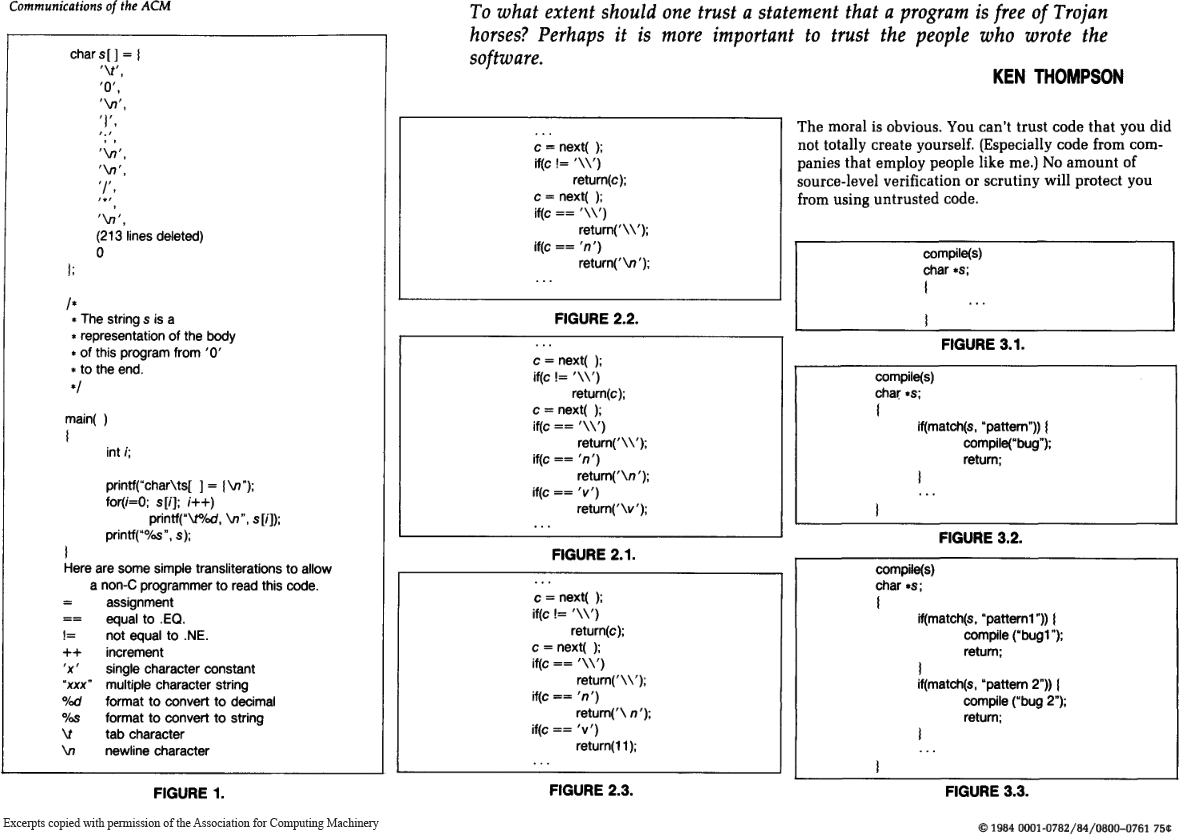
\includegraphics{assets/images/ken-thompson-hack.png}
  \caption{Trechos do artigo de Ken Thompson 'Reflexões sobre confiar na confiança'}
  \label{fig:ken-thompson-hack}
\end{figure}

Thompson demonstrou que mesmo se você tiver acesso ao código-fonte, seu compilador - ou qualquer outro programa ou hardware de gerenciamento de programa - pode estar comprometido e detectar esse backdoor seria muito difícil. Assim, na prática, um sistema verdadeiramente \textit{confiável} não existe. Você teria que criar todo o seu software \textit{e} todo o seu hardware (montadores, compiladores, vinculadores, etc.) a partir do zero, sem a ajuda de nenhum software externo ou maquinário auxiliado por software.

\begin{quotation}\begin{samepage}
\enquote{Se você deseja fazer uma torta de maçã do zero, você deve primeiro inventar o universo.}
\begin{flushright} -- Carl Sagan\footnote{Carl Sagan, \textit{Cosmos} \cite{cosmos}}
\end{flushright}\end{samepage}\end{quotation}

O hack do Ken Thompson é um backdoor particularmente engenhoso e difícil de detectar, então vamos dar uma olhada rápida em um backdoor difícil de ser detectado, que funciona sem modificar nenhum software. Os pesquisadores descobriram uma maneira de comprometer o hardware crítico de segurança alterando a polaridade das impurezas do silício.~\cite{becker2013stealthy} Apenas mudando as propriedades físicas das coisas de que os chips de computador são feitos, eles foram capazes de comprometer um gerador de números aleatórios criptograficamente seguro. Como essa mudança não pode ser encontrada, o backdoor não pode ser detectado por inspeção óptica, que é um dos mecanismos de detecção de violação mais importantes para chips como esses.

\begin{figure}
  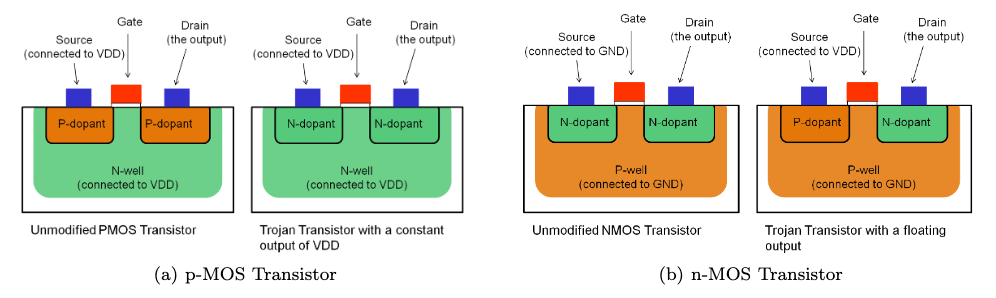
\includegraphics{assets/images/stealthy-hardware-trojan.png}
  \caption{Os Cavalos de Tróia Dopant-Level Escondidos no Hardware por Becker, Regazzoni, Paar, Burleson}
  \label{fig:stealthy-hardware-trojan}
\end{figure}

Parece assustador? Bem, mesmo se você fosse capaz de construir tudo do zero, ainda teria que confiar na matemática. Você teria que confiar que \textit{secp256k1} é uma curva elíptica que não possui nenhum tipo de backdoor ou erro. Sim, backdoors maliciosos podem ser inseridos nas bases matemáticas das funções criptográficas e, sem dúvida, isso já aconteceu pelo menos uma vez.~\cite{wiki:Dual_EC_DRBG} Existem boas razões para você ser paranóico e o fato de que tudo, desde o seu hardware, até seu software, passando pelas curvas elípticas utilizadas podem ter backdoors~\cite{wiki:backdoors}, são alguns dos motivos.

\begin{quotation}\begin{samepage}
\enquote{Não confie. Verifique.}
\begin{flushright} -- Bitcoinheiros de todos os lugares
\end{flushright}\end{samepage}\end{quotation}

Os exemplos acima devem ilustrar que a computação \textit{confiável} é utópica. O Bitcoin é provavelmente o sistema que mais se aproxima dessa utopia, mas ainda assim, é \textit{preciso um certo mínimo de confiança} --- com o objetivo de remover a confiança sempre que possível. Indiscutivelmente, a cadeia de confiança é interminável, já que você também terá que confiar que a computação requer energia, que P não é igual a NP e que você está realmente na realidade básica e não preso em uma simulação por agentes mal-intencionados.

Os desenvolvedores estão trabalhando em ferramentas e procedimentos para minimizar ainda mais qualquer confiança remanescente. Por exemplo, os desenvolvedores do Bitcoin criaram o Gitian \footnote{\url{https://gitian.org/}}, que é um método de distribuição de software para criar construções determinísticas. A ideia é que, se vários desenvolvedores forem capazes de reproduzir binários idênticos, a chance de adulteração maliciosa será reduzida. Os backdoors mais fantasiosos não são o único vetor de ataque. A simples chantagem ou extorsão também são ameaças reais. Como no protocolo principal, a descentralização é usada para minimizar a confiança.

Vários esforços estão sendo feitos para melhorar o problema do ovo e da galinha do bootstrapping, que o hack de Ken Thompson tão brilhantemente apontou~\cite{web:bootstrapping}. Um desses esforços é o Guix\footnote{\url{https://guix.gnu.org}} (a pronuncia correta é \textit{geeks}), que usa gerenciamento de pacote declarado funcionalmente levando a compilações reproduzíveis bit a bit por design. O resultado é que você não precisa mais confiar em nenhum servidor que fornece o software, pois pode verificar se o binário fornecido não foi adulterado, reconstruindo-o do zero. Recentemente, um pull request foi mesclado para integrar o Guix ao processo de build do Bitcoin.\footnote{Veja o PR 15277 do \texttt{bitcoin-core}: \url{https://github.com/bitcoin/bitcoin/pull/15277}}

\begin{figure}
  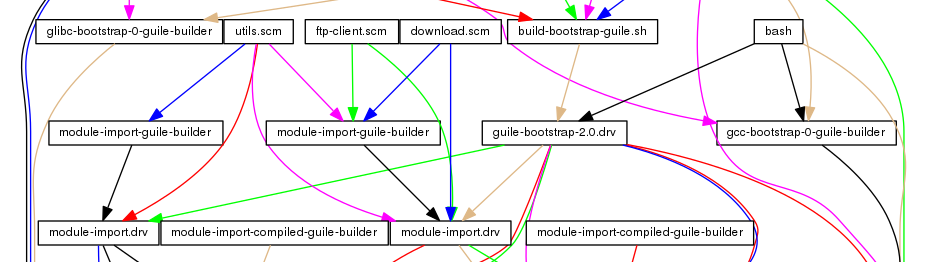
\includegraphics{assets/images/guix-bootstrap-dependencies.png}
  \caption{O que veio primeiro, o ovo ou a galinha?}
  \label{fig:guix-bootstrap-dependencies}
\end{figure}

Felizmente, o Bitcoin não depende de um único algoritmo ou peça de hardware. Um efeito da descentralização radical do Bitcoin é um modelo de segurança distribuído. Embora as backdoors descritos acima não devam ser desconsiderados, é improvável que cada software de carteira, cada carteira física, cada biblioteca criptográfica, cada implementação de node e cada compilador de cada linguagem sejam comprometidos. Possível, mas altamente improvável.

Observe que você pode gerar uma chave privada sem depender de nenhum hardware ou software computacional. Você pode jogar uma moeda ~\cite{antonopoulos2014mastering} algumas vezes, embora dependendo de sua moeda e estilo de lançamento esta fonte de aleatoriedade possa não ser suficientemente aleatória. Há um motivo pelo qual protocolos de armazenamento como Glacier\footnote{\url{https://glacierprotocol.org/}} aconselham o uso de dados de nível de cassino como uma das duas fontes de entropia.

O Bitcoin me forçou a refletir sobre o que realmente significa não confiar em ninguém. Isso aumentou minha consciência do problema do bootstrap e da cadeia de confiança implícita no desenvolvimento e execução de software. Isso também aumentou minha consciência sobre as muitas maneiras pelas quais software e hardware podem ser comprometidos.

\paragraph{O Bitcoin me ensinou a não confiar, mas a verificar.}

% ---
%
% #### Down the Rabbit Hole
%
% - [The Bitcoin whitepaper][Nakamoto] by Satoshi Nakamoto
% - [Reflections on Trusting Trust][\textit{Reflections on Trusting Trust}] by Ken Thompson
% - [51% Attack][majority] on the Bitcoin Developer Guide
% - [Bootstrapping][bootstrapping], Guix Manual
% - [Secp256k1][secp256k1] on the Bitcoin Wiki
% - [ECC Backdoors][backdoors], [Dual EC DRBG][has already happened] on Wikipedia
%
% [Emmanuel Boutet]: https://commons.wikimedia.org/wiki/User:Emmanuel.boutet
% [\textit{Reflections on Trusting Trust}]: https://www.archive.ece.cmu.edu/~ganger/712.fall02/papers/p761-thompson.pdf
% [found a way]: https://scholar.google.com/scholar?hl=en&as_sdt=0%2C5&q=Stealthy+Dopant-Level+Hardware+Trojans&btnG=
% [Gitian]: https://gitian.org/
% [bootstrapping]: https://www.gnu.org/software/guix/manual/en/html_node/Bootstrapping.html
% [Guix]: https://www.gnu.org/software/guix/
% [pull-request]: https://github.com/bitcoin/bitcoin/pull/15277
% [flip a coin]: https://github.com/bitcoinbook/bitcoinbook/blob/develop/ch04.asciidoc#private-keys
% [Glacier]: https://glacierprotocol.org/
% [secp256k1]: https://en.bitcoin.it/wiki/Secp256k1
% [majority]: https://bitcoin.org/en/developer-guide#term-51-attack
%
% <!-- Wikipedia -->
% [backdoors]: https://en.wikipedia.org/wiki/Elliptic-curve_cryptography#Backdoors
% [has already happened]: https://en.wikipedia.org/wiki/Dual_EC_DRBG
% [Carl Sagan]: https://en.wikipedia.org/wiki/Cosmos_%28Carl_Sagan_book%29
% [alice]: https://en.wikipedia.org/wiki/Alice%27s_Adventures_in_Wonderland
% [carroll]: https://en.wikipedia.org/wiki/Lewis_Carroll
